\section{Methodology}
\label{sec:methodology}

In this section, we rigorously formalize the semantic reconstruction threat model and define the SHArd Disclosure Estimator (SHADE). We subsequently detail the construction of the CoShard algorithm, demonstrating how it explicitly optimizes the trade-off between RAG utility and disclosure risk through a constrained graph partitioning objective.

\subsection{Formalizing the Semantic Vector Space}
Let $\mathcal{D} = \{d_1, d_2, \dots, d_n\}$ represent an enterprise knowledge base consisting of $n$ sensitive documents. In a standard Retrieval-Augmented Generation (RAG) pipeline, an embedding function $f_\theta : \mathcal{D} \to \mathbb{R}^d$, parameterized by a pre-trained neural encoder (e.g., \texttt{text-embedding-ada-002} or \texttt{BGE-large}), maps each discrete document $d_i$ to a dense, continuous vector representation $\mathbf{v}_i \in \mathcal{V}$, where $d$ is the dimensionality of the embedding space.

The geometric proximity of these vectors in $\mathbb{R}^d$ encodes their semantic similarity. Given a user query $q$, the RAG retriever projects $q$ into the same space to yield $\mathbf{q} = f_\theta(q)$, and retrieves the top-$k$ most similar documents by computing the cosine similarity:
\begin{equation}
\text{sim}(\mathbf{v}_i, \mathbf{q}) = \frac{\mathbf{v}_i \cdot \mathbf{q}}{\|\mathbf{v}_i\| \|\mathbf{q}\|}
\end{equation}

In a distributed RAG environment, the vector space $\mathcal{V}$ is partitioned across $m$ physically or logically isolated shards, $\mathcal{P} = \{S_1, S_2, \dots, S_m\}$, such that $\bigcup_{j=1}^m S_j = \mathcal{V}$ and $S_j \cap S_k = \emptyset$ for all $j \neq k$. At inference time, the query $\mathbf{q}$ is broadcast to a subset of shards, and the globally top-$k$ documents are aggregated and injected into the LLM context window.

\subsection{The Semantic Reconstruction Threat Model}
We assume an honest-but-curious adversary $\mathcal{A}$ who has successfully compromised a single shard $S_j$, or alternatively, is monitoring the local network traffic of an LLM agent querying $S_j$. The adversary's goal is to reconstruct a highly sensitive corporate topic $T \subset \mathcal{D}$ (e.g., an unannounced merger or a specific patient's comprehensive medical history).

Recent advancements in generative embedding inversion attacks, such as GEIA \cite{li2023geia} and Vec2Text \cite{morris2023vec2text}, have demonstrated that an adversary can reconstruct exact document text given access to its dense vector $\mathbf{v}_i$. However, reconstructing an isolated, fragmented sentence provides minimal actionable intelligence. To successfully reconstruct the comprehensive topic $T$, the adversary must observe a critical mass of semantically adjacent vectors belonging to $T$.

Let $C_T \subseteq \mathcal{V}$ represent the dense cluster of embeddings that semantically define topic $T$. We define a reconstruction threshold $\tau \in [0, 1]$. If the adversary observes a fraction of $C_T$ strictly greater than $\tau$ residing on their compromised shard $S_j$, they possess sufficient context to successfully prompt a generative inversion model to reconstruct the overarching intent of $T$. Mathematically, the attack succeeds if:
\begin{equation}
\max_{S_j \in \mathcal{P}} \frac{|C_T \cap S_j|}{|C_T|} > \tau
\end{equation}

\subsection{The SHArd Disclosure Estimator (SHADE)}
To mathematically quantify this vulnerability before an attack occurs, we introduce the SHArd Disclosure Estimator (SHADE). SHADE operates over a semantic similarity graph constructed from the embedding space.

We construct an undirected K-Nearest Neighbor (K-NN) graph $G = (V, E, W)$, where each node $v_i \in V$ represents a document embedding $\mathbf{v}_i$. An edge $(i, k) \in E$ exists if $\mathbf{v}_k$ is among the $K$ closest neighbors to $\mathbf{v}_i$ in the vector space. The weight of the edge, $w_{ik} \in W$, is defined by the exponential cosine similarity:
\begin{equation}
w_{ik} = \exp\left( \beta \cdot \text{sim}(\mathbf{v}_i, \mathbf{v}_k) \right)
\end{equation}
where $\beta$ is a temperature hyperparameter that accentuates highly confident semantic relationships.

The SHADE metric calculates the probability that two strongly connected semantic concepts (edges in $G$) are inadvertently co-located onto the exact same shard. Given a partition $\mathcal{P} = \{S_1, \dots, S_m\}$, let $\delta(i, k)$ be the Kronecker delta function, which equals $1$ if nodes $i$ and $k$ are assigned to the same shard $S_j$, and $0$ otherwise. The SHADE score for the partition $\mathcal{P}$ is the ratio of the sum of internal edge weights to the total sum of edge weights in the graph:
\begin{equation}
\text{SHADE}(\mathcal{P}) = \frac{\sum_{(i, k) \in E} w_{ik} \cdot \delta(i, k)}{\sum_{(i, k) \in E} w_{ik}}
\end{equation}

A SHADE score approaching $1.0$ indicates that highly related semantic topics are densely packed into single shards (typical of K-Means or GraphRAG). A SHADE score approaching $0.0$ indicates that semantic edges are uniformly fragmented across the network. 

We explicitly acknowledge that SHADE is a proxy metric structurally related to graph modularity. To ensure our privacy evaluation is mathematically independent from the utility graph, we introduce a second, orthogonal metric: the \textbf{Entity Leakage Rate (ELR)}. We define a set of known sensitive entities $\mathcal{E}$ (e.g., specific patient IDs or confidential project names). For each entity $e \in \mathcal{E}$, let $D_e \subset \mathcal{D}$ be the subset of documents mentioning $e$. The ELR measures the maximum concentration of any entity's documents within a single shard:
\begin{equation}
\text{ELR}(\mathcal{P}) = \frac{1}{|\mathcal{E}|} \sum_{e \in \mathcal{E}} \max_{S_j \in \mathcal{P}} \frac{|D_e \cap S_j|}{|D_e|}
\end{equation}
While SHADE acts as the differentiable heuristic used during algorithmic optimization, ELR serves as the independent ground-truth evaluation of reconstruction risk.

\subsection{The CoShard Objective Function}
While minimizing SHADE strictly reduces disclosure risk, it inherently destroys the semantic contiguity required by RAG retrievers, severely degrading retrieval utility (demonstrating an empirical privacy-utility trade-off). Therefore, CoShard explicitly formulates semantic sharding as a constrained multi-objective optimization problem.

To measure retrieval utility, we employ the standard Leiden modularity $Q$ \cite{ng2001spectral}, which measures the density of links inside communities compared to links between communities. The standard modularity for partition $\mathcal{P}$ is defined as:
\begin{equation}
Q(G, \mathcal{P}) = \frac{1}{2M} \sum_{i, k} \left( w_{ik} - \gamma \frac{d_i d_k}{2M} \right) \delta(i, k)
\end{equation}
where $M$ is the total sum of edge weights, $d_i$ is the weighted degree of node $i$, and $\gamma$ is the resolution parameter.

CoShard maximizes a novel penalized objective function, explicitly subtracting the SHADE metric weighted by a privacy constraint hyperparameter $\lambda \geq 0$:
\begin{equation}
\mathcal{O}_{\text{CoShard}} = Q(G, \mathcal{P}) - \lambda \cdot \text{SHADE}(\mathcal{P})
\label{eq:coshard_objective}
\end{equation}

By tuning $\lambda$, system administrators can dynamically trace the Pareto frontier. When $\lambda = 0$, CoShard collapses to standard Leiden modularity (maximizing utility, sacrificing privacy). As $\lambda \to \infty$, CoShard actively fractures semantic clusters, heavily prioritizing data security over retrieval coherence.

\subsection{The 2-Phase CoShard Algorithm}
Maximizing Equation \ref{eq:coshard_objective} is an NP-hard problem. We approximate the global maximum using a highly scalable, two-phase iterative heuristic, visualized in Figure \ref{fig:coshard_flowchart}.

\begin{figure}[htbp]
\centering
\begin{tikzpicture}[
    node distance=1.5cm and 2cm,
    box/.style={rectangle, draw, fill=blue!10, text width=3.5cm, text centered, rounded corners, minimum height=1cm, font=\small},
    decision/.style={diamond, draw, fill=red!10, text width=2.5cm, text centered, inner sep=0pt, font=\footnotesize},
    arrow/.style={thick,->,>=stealth}
]

% Nodes
\node (init) [box] {Initialize $G=(V,E)$ \\ Each node in own shard};
\node (phase1) [box, below=of init] {\textbf{Phase 1: Local Move}\\ Move $v_i$ to neighbor shard to maximize $\mathcal{O}$};
\node (check1) [decision, below=of phase1, yshift=-0.5cm] {Any node moved?};
\node (phase2) [box, right=of phase1] {\textbf{Phase 2: Aggregation}\\ Collapse shards into super-nodes};
\node (finish) [box, below=of check1, yshift=-0.5cm, fill=green!10] {Output final partitions $\mathcal{P}$};

% Arrows
\draw [arrow] (init) -- (phase1);
\draw [arrow] (phase1) -- (check1);
\draw [arrow] (check1) -- node[anchor=south] {Yes} (phase2);
\draw [arrow] (phase2) |- (phase1);
\draw [arrow] (check1) -- node[anchor=east] {No} (finish);

\end{tikzpicture}
\caption{Flowchart of the 2-Phase CoShard Algorithmic Pipeline. The system recursively alternates between local modularity optimization (penalized by SHADE) and graph contraction until convergence.}
\label{fig:coshard_flowchart}
\end{figure}

\begin{algorithm}[htbp]
\caption{The CoShard Partitioning Algorithm}
\renewcommand{\algorithmicrequire}{\textbf{Input:}}
\renewcommand{\algorithmicensure}{\textbf{Output:}}
\begin{algorithmic}[1]
\REQUIRE Similarity Graph $G=(V, E, W)$, Privacy Penalty $\lambda$
\ENSURE Partition assignments $\mathcal{P} = \{S_1, \dots, S_m\}$
\STATE Initialize each node $v_i$ into its own distinct shard: $S_i = \{v_i\}$
\STATE $\text{converged} \leftarrow \text{False}$
\WHILE{not converged}
    \STATE $\text{converged} \leftarrow \text{True}$
    \STATE \textit{// Phase 1: Local Optimization}
    \FOR{each node $v_i \in V$ in random order}
        \STATE Remove $v_i$ from its current shard $S_{curr}$
        \STATE Let $\mathcal{N}(v_i)$ be the set of shards containing neighbors of $v_i$
        \STATE $S_{best} \leftarrow \emptyset$
        \STATE $\Delta \mathcal{O}_{max} \leftarrow 0$
        \FOR{each candidate shard $S_c \in \mathcal{N}(v_i)$}
            \STATE Calculate $\Delta Q$, the change in Modularity if $v_i \to S_c$
            \STATE Calculate $\Delta \text{SHADE}$, the change in Disclosure Risk
            \STATE $\Delta \mathcal{O} \leftarrow \Delta Q - \lambda \cdot \Delta \text{SHADE}$
            \IF{$\Delta \mathcal{O} > \Delta \mathcal{O}_{max}$}
                \STATE $\Delta \mathcal{O}_{max} \leftarrow \Delta \mathcal{O}$
                \STATE $S_{best} \leftarrow S_c$
            \ENDIF
        \ENDFOR
        \IF{$\Delta \mathcal{O}_{max} > 0$}
            \STATE Assign $v_i \to S_{best}$
            \STATE $\text{converged} \leftarrow \text{False}$
        \ELSE
            \STATE Return $v_i \to S_{curr}$
        \ENDIF
    \ENDFOR
    \STATE \textit{// Phase 2: Graph Aggregation}
    \IF{not converged}
        \STATE Contract $G$: group nodes in the same shard into super-nodes
        \STATE Sum edge weights between corresponding super-nodes
    \ENDIF
\ENDWHILE
\STATE \textbf{return} $\mathcal{P}$
\end{algorithmic}
\label{alg:coshard}
\end{algorithm}

As detailed in Algorithm \ref{alg:coshard}, Phase 1 evaluates the local move of every node $v_i$ to a neighboring shard. The move is only accepted if the increase in semantic cohesion ($\Delta Q$) outweighs the resulting privacy penalty ($\lambda \cdot \Delta \text{SHADE}$). Phase 2 contracts the graph by collapsing identical shard assignments into super-nodes, reducing the search space and allowing the algorithm to iteratively scale to massive enterprise corpora with millions of embeddings.

\subsection{Visualizing the Partition Pipeline}
To intuitively understand the CoShard routing mechanism, consider a subset of highly connected medical queries (Figure \ref{fig:pipeline_overview}).

\begin{figure*}[htbp]
\centerline{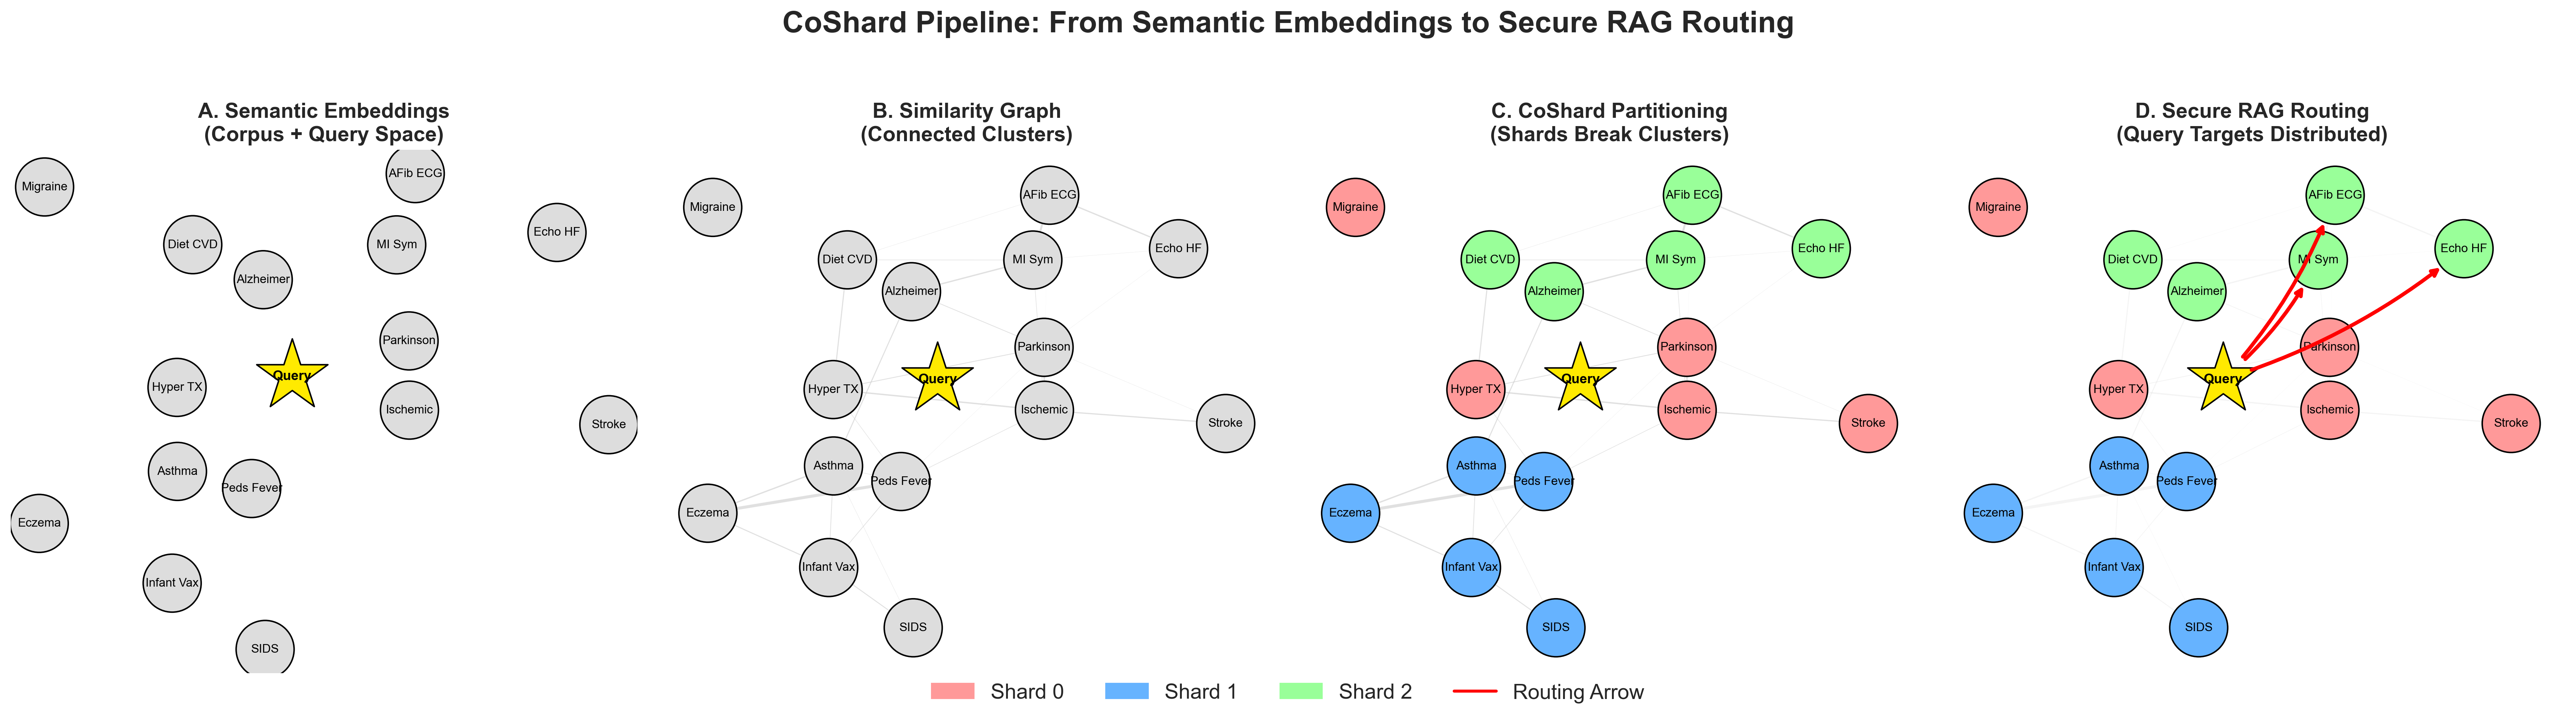
\includegraphics[width=\textwidth]{figures/pipeline_overview.png}}
\caption{The complete CoShard pipeline. (A) Raw documents and the User Query are embedded into semantic space. (B) A K-NN similarity graph connects highly related topics. (C) The CoShard algorithm explicitly forces connected clusters into different shards (colors) to minimize the SHADE disclosure penalty. (D) At inference, a User Query is safely routed to documents distributed across multiple shards, preventing any single shard from inferring the full topic.}
\label{fig:pipeline_overview}
\end{figure*}
